\documentclass[tikz,border=10pt]{standalone}
\usepackage{helvet}
\renewcommand{\familydefault}{\sfdefault}
\usepackage{amsmath}
\usepackage{tikz}
\usetikzlibrary{positioning, fit, calc, arrows.meta, shapes.geometric, backgrounds}

% Define Colors
\definecolor{emeraldpine}{HTML}{1A4D3E}
\definecolor{harvardcrimson}{HTML}{A51C30}
\definecolor{ethdarkblue}{HTML}{1F407A}
\definecolor{ethpetrol}{HTML}{007A87}
\definecolor{ethbronze}{HTML}{B87333}
\definecolor{ethpurple}{HTML}{5B4B8A}
\definecolor{ink}{HTML}{1A202C}
\definecolor{softink}{HTML}{4A5568}
\definecolor{paleink}{HTML}{A0AEC0}
\definecolor{cardbg}{HTML}{F8FAFC}
\definecolor{shadecolor}{HTML}{F4F6F9}

\begin{document}
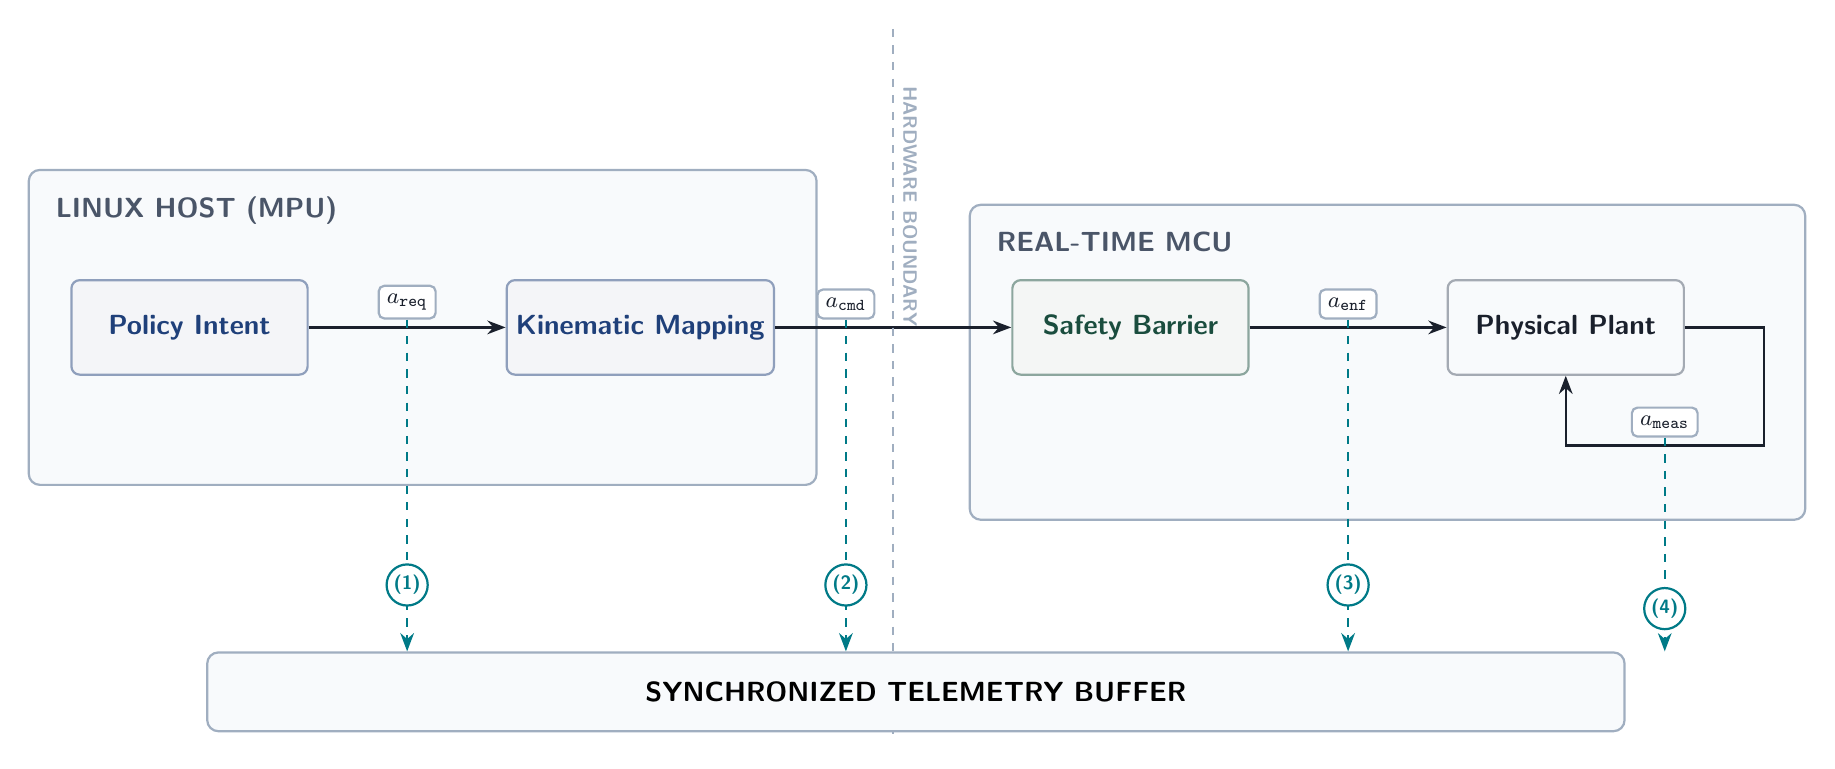
\begin{tikzpicture}[
    font=\sffamily,
    >=Stealth,
    node distance=2.5cm,
    block/.style={
        rectangle, 
        draw=ethdarkblue!50, 
        fill=shadecolor,
        thick, 
        rounded corners=3pt, 
        minimum width=3cm, 
        minimum height=1.2cm, 
        align=center,
        text=ink,
        font=\bfseries
    },
    plant/.style={
        block,
        draw=softink!50,
        fill=cardbg,
    },
    safety/.style={
        block,
        draw=emeraldpine!50,
        fill=emeraldpine!5,
        text=emeraldpine
    },
    intent/.style={
        block,
        draw=ethdarkblue!50,
        fill=ethdarkblue!5,
        text=ethdarkblue
    },
    computedomain/.style={
        rectangle,
        draw=paleink,
        fill=cardbg,
        rounded corners=4pt,
        thick,
        inner sep=15pt
    },
    tap/.style={
        circle,
        solid,
        draw=ethpetrol,
        fill=white,
        thick,
        inner sep=1pt,
        minimum size=0.5cm,
        font=\scriptsize\bfseries,
        text=ethpetrol
    },
    signal/.style={
        rectangle,
        fill=white,
        draw=paleink,
        rounded corners=2pt,
        inner sep=3pt,
        font=\footnotesize\ttfamily\bfseries
    }
]

% Nodes
\node[intent] (intent) {Policy Intent};
\node[intent, right=2.5cm of intent] (kinematic) {Kinematic Mapping};
\node[safety, right=3cm of kinematic] (safety) {Safety Barrier};
\node[plant, right=2.5cm of safety] (plant) {Physical Plant};

% Signals along path
\draw[->, thick, ink] (intent) -- node[signal, midway, above=0.1cm] (areq) {$a_{\text{req}}$} (kinematic);
\draw[->, thick, ink] (kinematic) -- node[signal, pos=0.3, above=0.1cm] (acmd) {$a_{\text{cmd}}$} (safety);
\draw[->, thick, ink] (safety) -- node[signal, midway, above=0.1cm] (aenf) {$a_{\text{enf}}$} (plant);

% Feedback
\draw[->, thick, ink] (plant.east) -- ++(1,0) -- ++(0,-1.5) coordinate (br) -- (br -| plant.south) node[signal, midway, above=0.1cm] (ameas) {$a_{\text{meas}}$} -- (plant.south);

% Domains
\begin{scope}[on background layer]
    \node[computedomain, fit=(intent) (kinematic) (areq), minimum height=4cm, label={[anchor=north west, inner sep=10pt, font=\bfseries\color{softink}]north west:LINUX HOST (MPU)}] (mpu) {};
    \node[computedomain, fit=(safety) (plant) (ameas) (br), minimum height=4cm, label={[anchor=north west, inner sep=10pt, font=\bfseries\color{softink}]north west:REAL-TIME MCU}] (mcu) {};
\end{scope}

% Hardware Boundary
\draw[dashed, thick, paleink] ($(mpu.north east)!0.5!(mcu.north west) + (0, 2)$) -- ($(mpu.south east)!0.5!(mcu.south west) - (0, 3)$) node[pos=0.25, sloped, above, font=\scriptsize\bfseries\color{softink}] {HARDWARE BOUNDARY};

% Telemetry Buffer
\node[rectangle, draw=paleink, thick, fill=cardbg, rounded corners=4pt, minimum width=18cm, minimum height=1cm, below=3.5cm of kinematic, xshift=3.5cm] (buffer) {\textbf{SYNCHRONIZED TELEMETRY BUFFER}};

% Taps
\draw[->, dashed, thick, ethpetrol] (areq.south) -- (areq.south |- buffer.north) node[tap, pos=0.8] {(1)};
\draw[->, dashed, thick, ethpetrol] (acmd.south) -- (acmd.south |- buffer.north) node[tap, pos=0.8] {(2)};
\draw[->, dashed, thick, ethpetrol] (aenf.south) -- (aenf.south |- buffer.north) node[tap, pos=0.8] {(3)};
\draw[->, dashed, thick, ethpetrol] (ameas.south) -- (ameas.south |- buffer.north) node[tap, pos=0.8] {(4)};

\end{tikzpicture}
\end{document}
